%-------------------------------------------------------------
% $Id$
% © Juan A. de la Puente, 2008
%-------------------------------------------------------------
\chapter{Cartas náuticas}
\label{ch:cartas}
%===================================
\section{Cartas náuticas }

\index{cartas náuticas|textbf}

\index{carta|textbf}
\index{carta!náutica}
\index{carta!electrónica}
\index{visor}
\index{plotter|textbf}
\index{avisos a los navegantes}
\index{Instituto Hidrográfico de la Marina|textbf}

Una carta náutica es un mapa de una zona de la superficie del mar y de la costa adyacente.
Las cartas muestran la forma de la costa, la profundidad del mar, los puntos peligrosos para 
la navegación, las ayudas a la navegación, los puntos relevantes de la costa, y todos los 
detalles útiles para navegar en la zona que cubren. 

Las cartas pueden presentarse de distintas formas. La más común es la carta impresa 
sobre una superficie de papel, pero cada vez son más frecuentes las \emph{cartas electrónicas}, 
cuyo contenido está codificado en forma numérica y almacenado en un dispositivo electrónico adecuado. Las cartas electrónicas no son simplemente una versión digital de las cartas 
en papel, sino que pueden contener información adicional, que se puede consultar de distintas formas, y mezclar con los datos obtenidos de otros instrumentos electrónicos. Para 
leer las cartas electrónicas se necesita un visor adecuado, que puede ser un computador 
ordinario dotado de los programas necesarios. Sin embargo es muy frecuente que las cartas electrónicas 
se utilicen con un computador especializado (\emph{plotter}) integrado con otros instrumentos electrónicos, como 
navegadores por satélite o sistemas de radar. 

Los servicios hidrográficos de cada país realizan los trabajos necesarios para recopilar 
los datos necesarios para confeccionar cartas de las zonas de navegación que les interesan, 
y publican cartas oficiales basadas en esos datos y en los que intercambian con otros países. Estos mismos servicios o, en ocasiones, editoriales privadas publican también cartas 
especialmente adaptadas a la navegación deportiva. Es muy importante mantener las cartas 
al día, aplicándoles las correcciones que se publican en los avisos a los navegantes o en 
otras publicaciones similares. En España el Instituto Hidrográfico de la Marina es el organismo encargado de publicar las cartas náuticas oficiales y otros documentos destinados a los navegantes.

%------------------------------------------------------------


\subsection{La proyección de Mercator}

\index{proyección|textbf}
\index{proyección!de Mercator|textbf}
\index{proyección!equivalente}
\index{proyección!isogónica}
\index{proyección!conforme}
\index{línea!ortodrómica}
\index{línea!loxodrómica}
\index{carta!mercatoriana|textbf}



La representación de la superficie de la Tierra, aproximadamente esférica, sobre una superficie plana se realiza mediante una \emph{proyección}. Una proyección es una relación que hace 
corresponder a cada punto de la superficie terrestre un punto del plano de la carta.%
\footnote{En términos matemáticos este tipo de relación se llama \emph{aplicación}. Para construir un mapa de 
forma correcta la aplicación debe ser \emph{biyectiva}, es decir a cada punto de la parte de la superficie terrestre considerada debe corresponder un único punto en la carta y viceversa.}
 Generalmente se procura que la proyección utilizada tenga determinadas características, como la 
conservación de las formas de los accidentes geográficos (proyecciones conformes), de las superficies de los mares y continentes (proyecciones equivalentes), etc. Ninguna proyección 
permite mantener todas estas propiedades a la vez, por lo que generalmente es necesario 
sacrificar algún aspecto de la realidad para representar adecuadamente otros. En el caso 
de la navegación marítima es fundamental que los ángulos medidos en la carta sean iguales que los medidos en la realidad, ya que, como veremos, muchas técnicas de navegación 
se basan en la medida de los ángulos que forman determinadas líneas. 
Una proyección que tiene esta propiedad es una \emph{proyección conforme}. 

\begin{figure}[hbtp]
\begin{center}
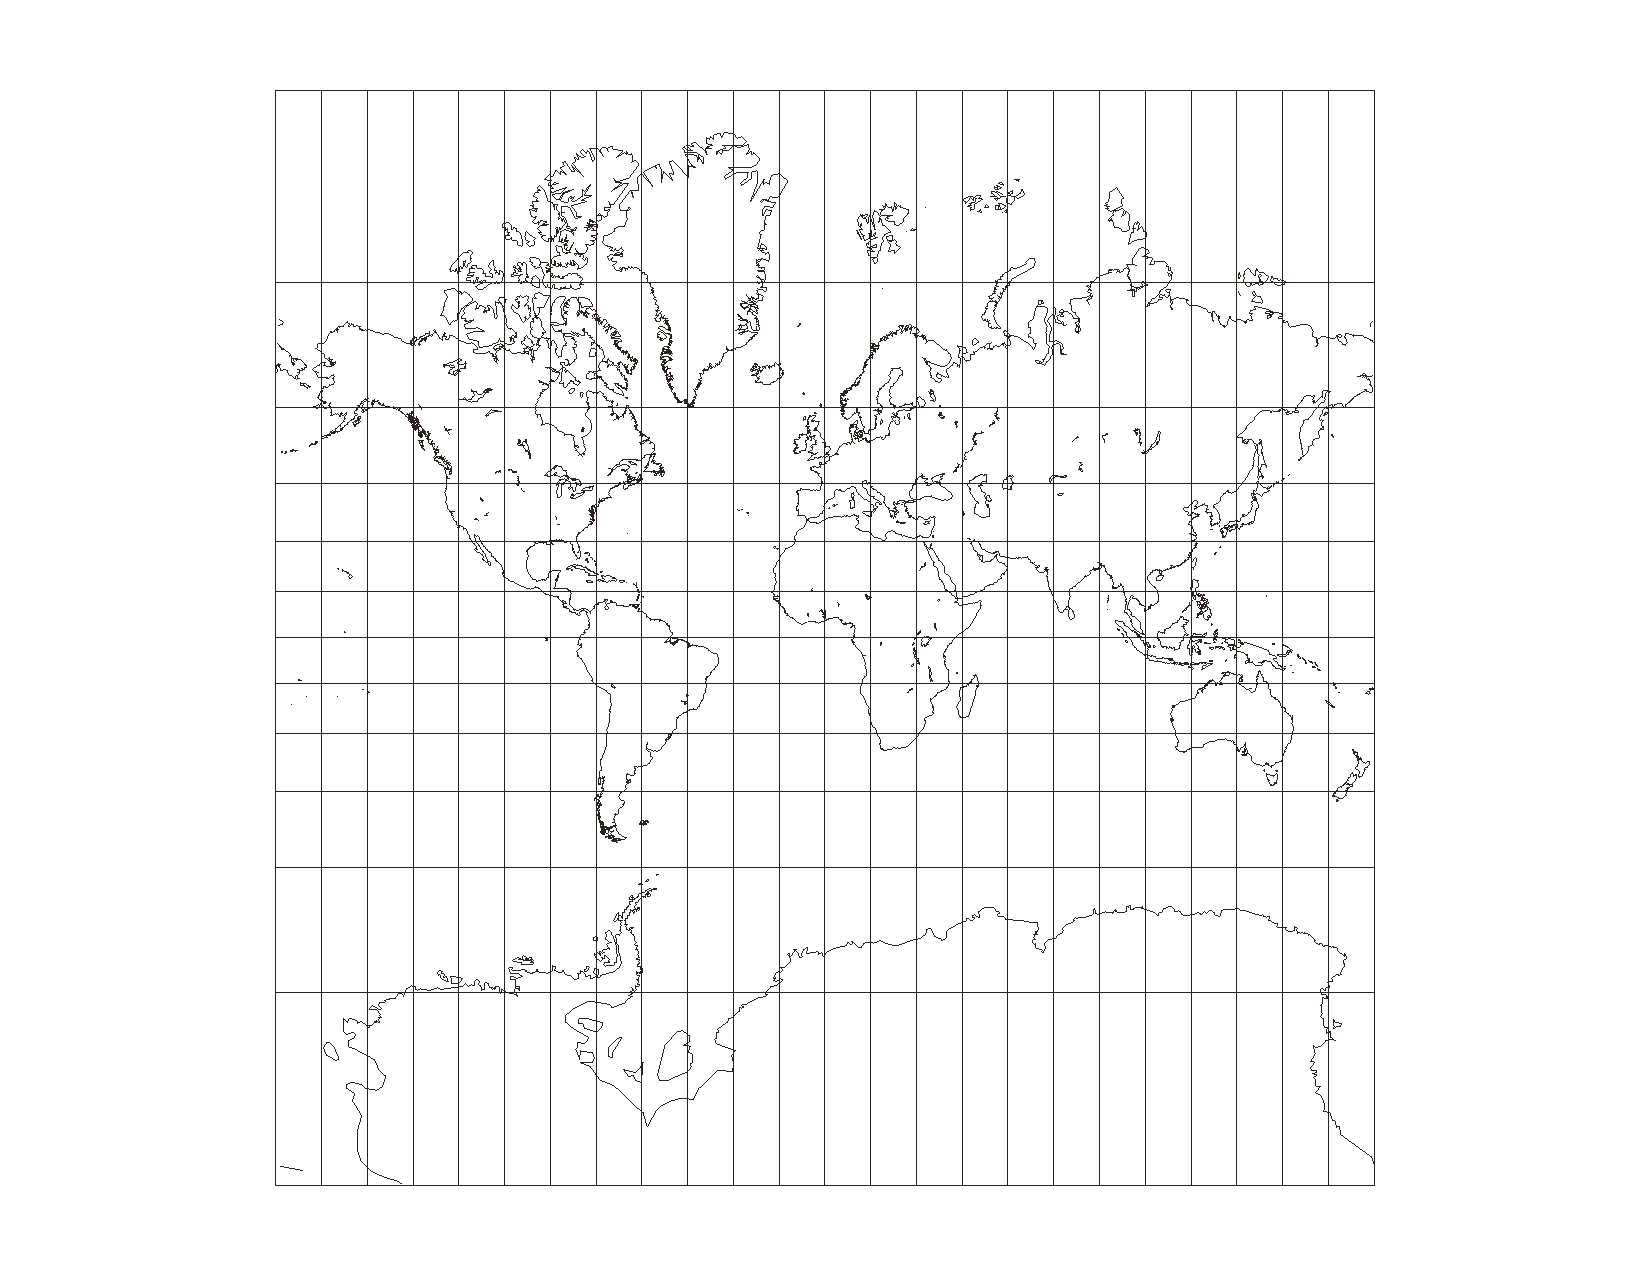
\includegraphics[scale=0.7]{mercator}\\
\caption{Mapamundi en proyección de Mercator.}
\label{fg:mercator}
\end{center}
\end{figure}

La proyección de Mercator, ideada en 1569 por el cartógrafo flamenco Gerhard Kremer,%
\footnote{El nombre «Kremer » significa «mercader». «Mercator » es una versión latinizada de este 
nombre.}
 es la que se utiliza para confeccionar la gran mayoría de las cartas náuticas. Es una 
proyección conforme, en la que los meridianos se representan como líneas verticales, y 
los paralelos como líneas horizontales (figura\ref{fg:mercator}). Todos los demás círculos máximos 
(líneas ortodrómicas) se representan mediante curvas. Por el contrario, las líneas que 
siguen un rumbo constante (loxodrómicas) se representan como líneas rectas. Como 
hemos visto, esta es la propiedad más importante de esta proyección desde el punto de 
vista de la navegación. Sin embargo, la proyección de Mercator tiene el inconveniente de 
que la superficie de los continentes e islas resulta alterada, de tal manera que las 
tierras situadas en latitudes altas aparecen aumentadas con respecto a las situadas cerca del 
Ecuador. Así, Groenlandia aparece en las cartas mercatorianas con un tamaño similar al de 
África, cuando en realidad ésta es mucho mayor. 

%-------------------------------------------------------------------------------
\subsection{Escala de las cartas }

\index{carta!escala|textbf}
\index{escala|textbf}
\index{escala!\textemdash|seealso{carta}}

La escala de una carta es la relación entre el tamaño de los objetos representados en la 
carta y el tamaño real de los mismos en la superficie de la Tierra. Por ejemplo, si la escala 
es $1/100\,000$, una línea de 1~cm en la carta representa una distancia real de 1~km 
($=100\,000\,\mbox{cm}$). Por tanto, cuanto mayor es la escala de una carta, con mayor detalle se 
representará en ella la superficie terrestre.%
\footnote{Puesto que la escala se representa mediante una fracción cuyo numerador es igual a la unidad, 
será tanto mayor cuanto menor sea el valor del denominador. Así, una escala de $1/50\,000$ es 
mayor que una de $1/100\,000$. }

\begin{figure}[hbtp]
\begin{center}
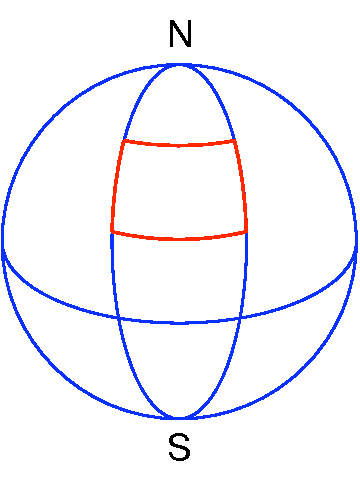
\includegraphics[scale=0.45]{convergencia}\\
\caption{Convergencia de los meridianos.}
\label{fg:convergencia}
\end{center}
\end{figure}

En las cartas mercatorianas  la escala  no es uniforme,  sino que aumenta con la latitud. La razón de ello estriba en la necesidad de que la proyección sea conforme. Mientras que un arco de meridiano de 1'  mide lo mismo en todas las latitudes (1milla náutica),%
\footnote{Salvo una pequeña diferencia debida a la falta de esfericidad de la Tierra.}
un arco de paralelo de 1' sólo sólo mide 1 milla en el Ecuador. A medida que se avanza hacia latitudes más 
altas, los meridianos se van acercando (figura~\ref{fg:convergencia}), por lo que la longitud de los paralelos 
va disminuyendo con la latitud, de tal manera que en la latitud $\phi$ la longitud de un arco de 
1’ de paralelo es igual a $\cos \phi$ millas. Como en la proyección de Mercator la separación entre las líneas rectas que representan los meridianos es constante e independiente de la latitud,  es necesario aumentar la escala en el sentido de la latitud para mantener la proporción entre la medida de los arcos de meridiano y de paralelo en todas las latitudes.
Ésta es la razón por la cual las tierras situadas cerca de los Polos parecen mayores que las que están cerca del Ecuador. 

La figura \ref{fg:escalas-lat-long} muestra la representación en una carta mercatoriana de un rectángulo de 
1’ de latitud por 1’ de longitud. La relación entre la medida en la carta de los lados del rectángulo es $y = x/\cos \phi$,
siendo $\phi$ la latitud del lado inferior. 
Para diferentes latitudes tenemos:
\[ 
\begin{array}{rr}
\multicolumn{1}{c}{\phi} & y \\ \hline
0º & x \\
30º & 1.15 x\\
45º & 1.41 x \\
60º & 2.00 x\\
\end{array}
\]
Por tanto, cuanto mayor sea la latitud tanto mayor será la relación entre el lado vertical y el horizontal del rectángulo. Como la longitud del lado vertical es siempre la misma, 1~milla, vemos que la escala aumenta con la latitud.

\begin{figure}[hbtp]
\begin{center}
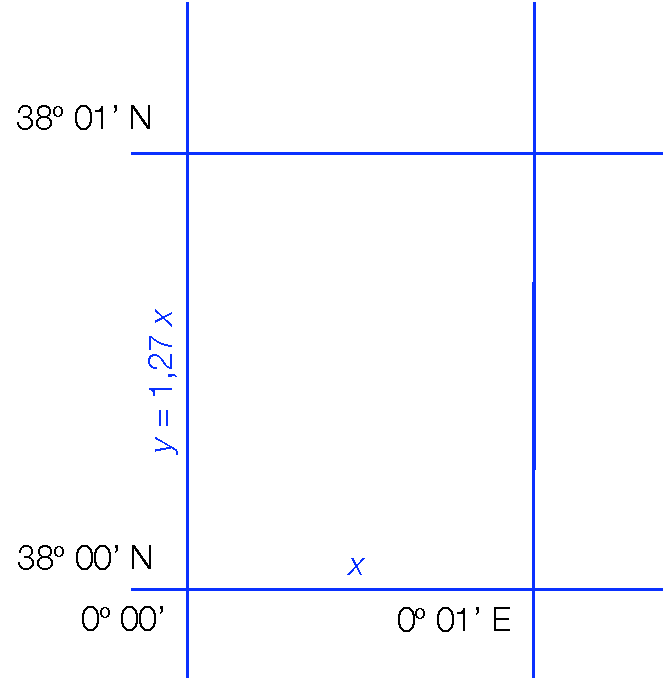
\includegraphics[scale=0.50]{escalas-lat-long}\\
\caption{Escalas de latitud y longitud.}
\label{fg:escalas-lat-long}
\end{center}
\end{figure}

%------------------------------------------------------------
\subsection{Otras proyecciones}

\index{proyección!gnomónica}
\index{proyección!gnomónica polar}
\index{proyección!polar estereográfica}
\index{proyección!de Lambert}
\index{derrota!ortodrómica}

La proyección de Mercator no es adecuada para representar las zonas polares, ya que por 
encima de los 60º de latitud la distorsión introducida por el aumento de la escala es muy 
grande, y los Polos no tienen representación. Por este motivo en las cartas de estas zonas 
se utilizan otras proyecciones, de las que la más común es la \emph{proyección gnomónica}. Ésta 
consiste en proyectar geométricamente la superficie terrestre desde el centro de la Tierra 
sobre un plano tangente a la misma. Cuando el punto de tangencia coincide con uno de los 
polos terrestres se denomina \emph{proyección gnomónica polar}. En este caso los meridianos se 
representan como rectas convergentes en el Polo, y los paralelos como circunferencias 
concéntricas con centro en el Polo. Otras proyecciones de uso frecuente en las cartas de las 
zonas polares son la \emph{proyección polar estereográfica} y la 
\emph{proyección de Lambert modificada}. 

La proyección gnomónica tiene la propiedad de que todos los círculos máximos se 
representan en las cartas como líneas rectas. Por este motivo a veces se usan cartas en pro- 
yección gnomónica oblicua (es decir, con el punto de tangencia en un lugar cualquiera de 
la superficie terrestre) para trazar derrotas ortodrómicas, es decir las que siguen un arco 
de círculo máximo. 

%===================================
\section{Características de las cartas}

\index{cartas náuticas!características}

Las cartas náuticas contienen numerosos detalles interesantes para la navegación, por lo 
que a veces su lectura puede resultar complicada a primera vista. Es necesario, por tanto, 
conocer los convenios de signos, rotulación, escalas, etc. que se utilizan en su confección, 
así como los procedimientos adecuados para mantenerlas al día. A continuación se resumen las características más importantes de las cartas oficiales españolas publicadas por el 
IHM (Instituto Hidrográfico de la Marina), que son similares a las de otros organismos. 
Características generales  

%--------------------------------------------------------------
\subsection{Identificación }

\index{cartas náuticas!identificación}

Las cartas náuticas se identifican mediante un número, que aparece en la esquina inferior 
derecha y en la superior izquierda de cada carta. Cerca del número situado en la esquina 
inferior derecha aparece también el número y la fecha de la edición, y la fecha de la última 
corrección efectuada en el momento de adquirir la carta (figura \ref{fg:id-carta}). 

\begin{figure}[htbp]
\begin{center}
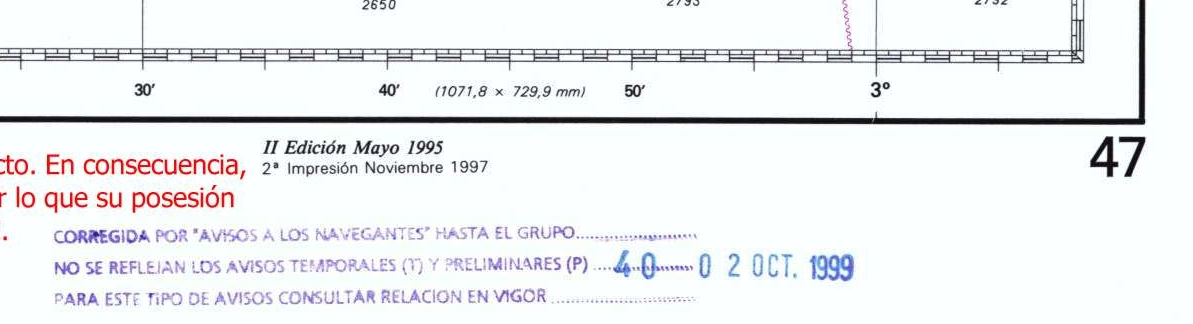
\includegraphics[width=\textwidth]{numero-carta}\\
\caption{Datos de identificación de la carta número 47 del IHM.}
\label{fg:id-carta}
\end{center}
\end{figure}

%--------------------------------------------------------------
\subsection{Tarjeta}
 
\index{cartas náuticas!características}

La mayoría de la información general sobre la carta se encuentra en la \emph{tarjeta}, que es la 
parte de la carta donde se describe la zona que abarca la carta, junto con otros datos de 
interés (figura \ref{fg:tarjeta}). 

\begin{figure}[hbtp]
\begin{center}
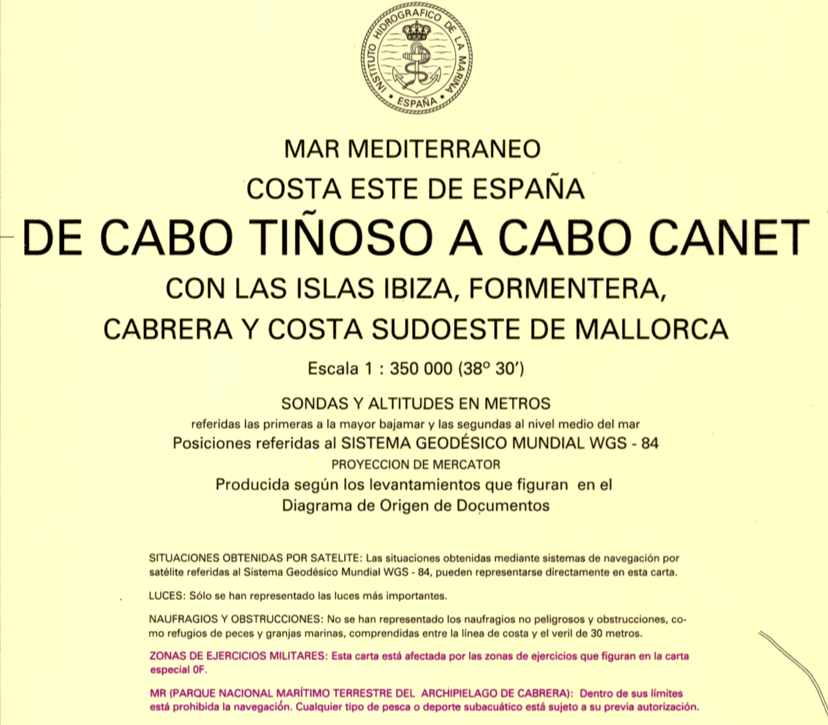
\includegraphics[width=\textwidth]{tarjeta}\\
\caption{Tarjeta de la carta número 47 del IHM.}
\label{fg:tarjeta}
\end{center}
\end{figure}

%--------------------------------------------------------------
\subsection{Escala}

\index{carta!escala}
\index{escala}

La escala de la carta es, como hemos visto, la relación entre el tamaño de los objetos 
representados en la carta y su tamaño real sobre la superficie terrestre. Como en la proyección de Mercator la escala varía con la latitud, la escala que figura en la tarjeta se 
refiere siempre a una latitud determinada. Las cartas tienen también escalas gráficas de 
latitudes y longitudes en sus bordes, que permiten leer las coordenadas de un punto cualquiera y medir distancias, tal como se explica más adelante. Por ejemplo, la escala de la 
carta nº 47 del IHM es de 1:350 000 en la latitud 38º 30’ N (figura \ref{fg:tarjeta}). En esta misma 
carta, la escala es ligeramente mayor en latitudes más altas, y ligeramente menor en latitudes más bajas. 

\subsubsection{Escalas de latitudes y longitudes }

\index{carta!escala gráfica}
\index{escala!gráfica}

Las cartas náuticas llevan dos tipos de escalas gráficas, que se utilizan para medir coordenadas y distancias (figura \ref{fg:escala-grafica}): 
\begin{itemize}
\item La \emph{escala de latitudes} está situada en los bordes laterales de la carta. Se usa para 
medir la latitud de un punto en la carta. También se usa para medir distancias, ya 
que 1~M = 1’ de latitud. 
\item \emph{La escala de longitudes} está situada en los bordes superior e inferior. Se usa para 
medir longitudes sobre la carta. 
\end{itemize}

\begin{figure}[hbtp]
\begin{center}
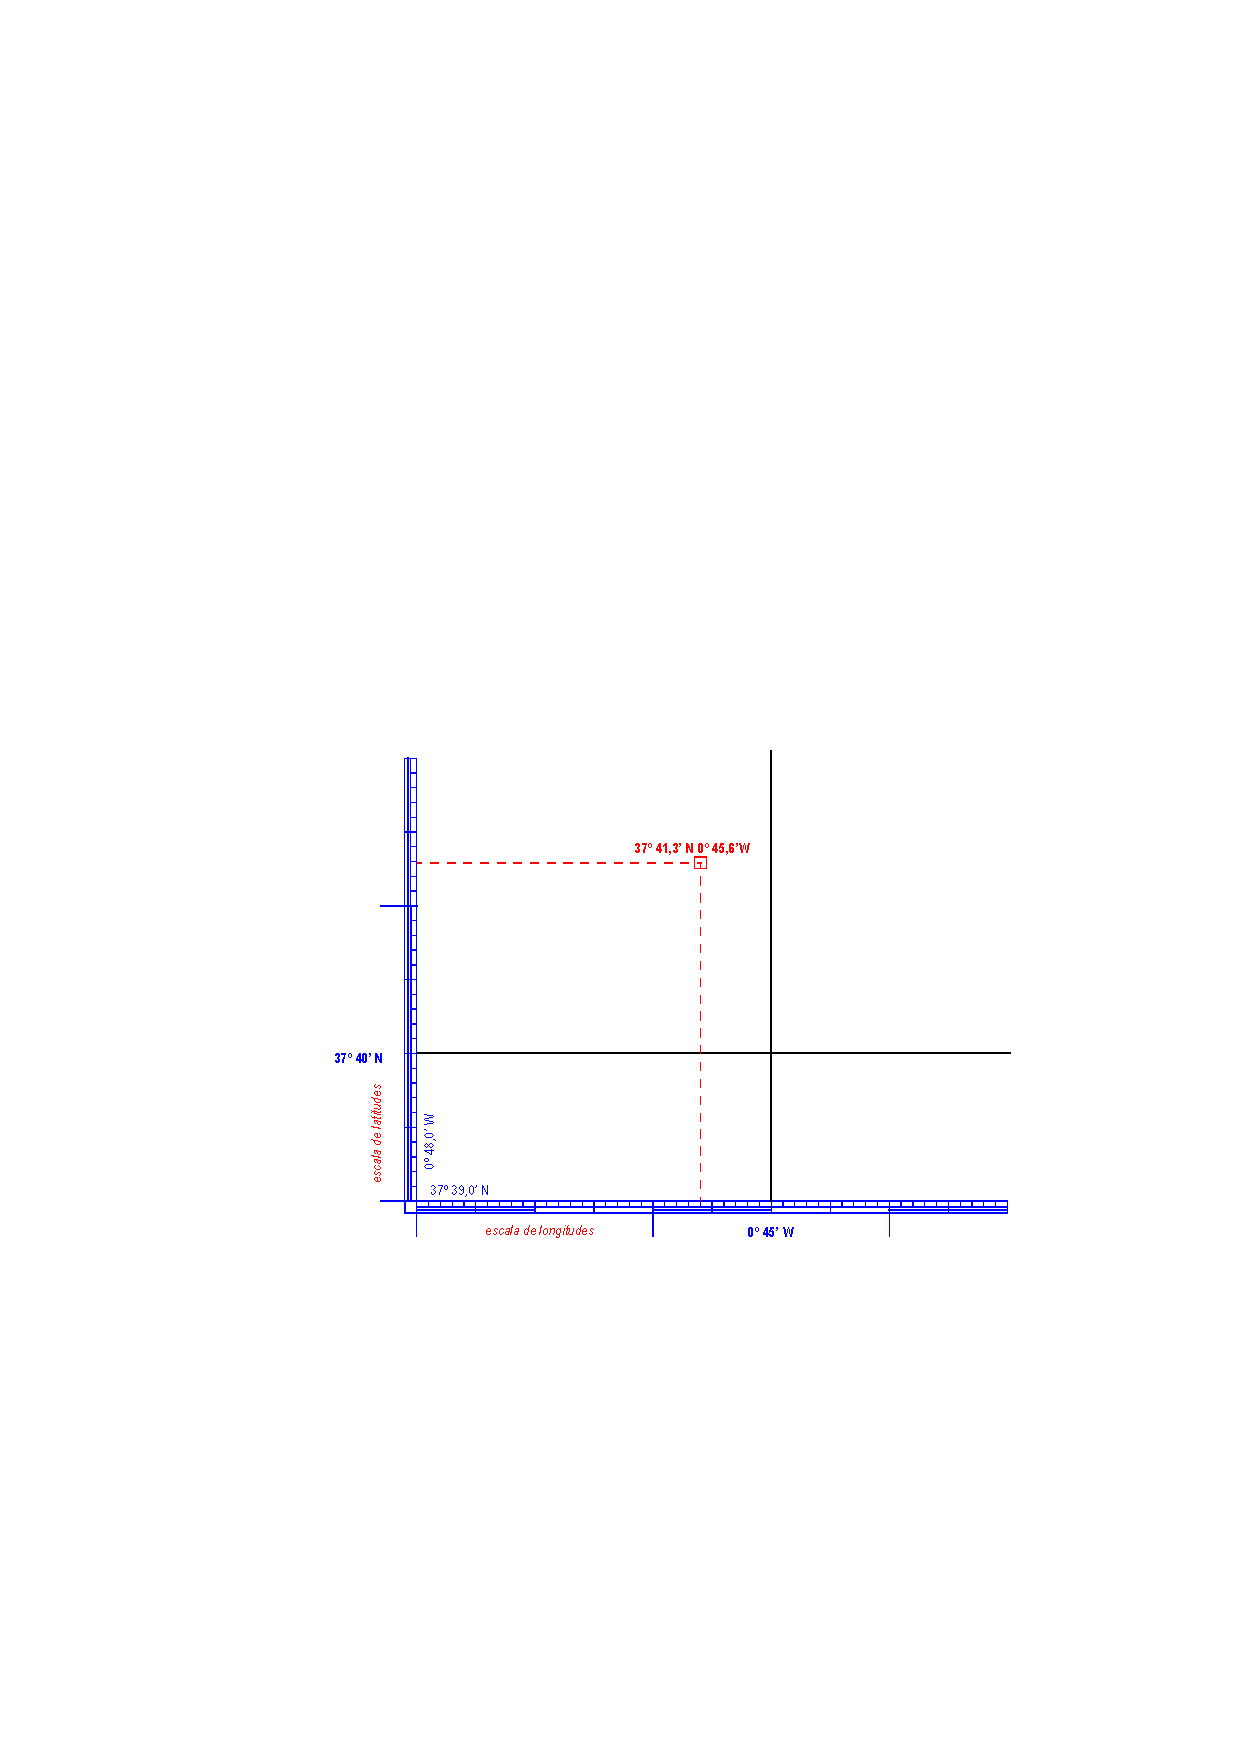
\includegraphics[width=\textwidth]{escala-grafica}\\
\caption{Escalas de latitud y longitud.}
\label{fg:escala-grafica}
\end{center}
\end{figure}

\begin{ejemplo}
El punto marcado en la carta de la figura  \ref{fg:escala-grafica} está situado en 37º 41,3’ N  0º 45,6’ W.
\end{ejemplo}

%--------------------------------------------------------------
\subsection{Tipos de cartas}

\index{cartas náuticas!tipos}
\index{cartas!generales}
\index{cartas!de arrumbamiento|seealso{cartas de recalada}}
\index{cartas!de recalada}
\index{cartas!de navegación costera}
\index{aproche}
\index{portulano}
\index{carta!cartucho}

Las cartas se clasifican según su escala y la superficie de la Tierra que representan en: 
\begin{itemize}
\item \emph{Cartas generales}: las que representan una gran extensión de la superficie de la 
Tierra, con escalas comprendidas entre 1:30\,000\,000 y 1:3\,000\,000.Se utilizan 
únicamente para trazar grandes derrotas en navegación oceánica. 
\item \emph{Cartas de arrumbamiento} o \emph{recalada}: representan una extensión limitada de la 
superficie terrestre, con una escala comprendida entre 1:3\,000\,000 y 1:200\,000. 
Se utilizan para navegar en distancias medias o para acercarse a la costa después 
de una navegación de altura. 
\item \emph{Cartas para navegación costera}: representan de forma detallada una porción de 
costa, con una escala comprendida entre 1:200\,000 y 1: 50\,000. 
\item \emph{Aproches}: son cartas de gran escala (del orden de 1:25\,000), que se utilizan para 
navegar cerca de los puertos o en zonas de gran dificultad. 
\item  \emph{Portulanos}: con escala mayor de 1:25\,000. Representan con gran detalle el interior 
de los puertos, canales y fondeaderos. 
\end{itemize}
Los aproches y portulanos se encuentran a menudo insertados en forma de 
\emph{cartucho} en otras cartas de menor escala. 

\index{cartas!de punto menor}
\index{cartas!de punto mayor}

También se habla de cartas de \emph{punto menor} o de \emph{punto mayor}. Se consideran cartas de 
punto menor las cartas generales y las de arrumbamiento, y cartas de punto mayor las restantes. 

%--------------------------------------------------------------
\subsection{Datum de la carta} 

\index{datum}
\index{datum!horizontal}

\index{datum!europeo (Potsdam)}
%\index{sistema geodésico mundial|see{WGS84}}
%\index{World Geodetic System|see{WGS84}}
\index{coordenadas!geográficas}
 
La tarjeta también contiene información sobre el \emph{datum horizontal} de la carta. Como 
vimos en el capítulo \ref{ch:introduccion}, este término se refiere al sistema de referencia que 
que se utiliza para determinar las coordenadas geográficas sobre la superficie de la Tierra. 
Actualmente las cartas españolas se refieren al \emph{sistema geodésico mundial} (WGS\,84), 
que es el que se utiliza en la mayoría de los países y 
en los sistemas de navegación por satélite  (ver capítulo \ref{ch:satelite}). Sin embargo, todavía se encuentran cartas referidas al  \emph{datum europeo de 1950}. Con el fin de permitir el uso de estas cartas en la navegación por satélite, la tarjeta proporciona instrucciones para convertir las coordenadas geográficas medidas en la carta al sistema WGS84 y 
viceversa. 

%\begin{figure}[hbtp]
%\begin{center}
%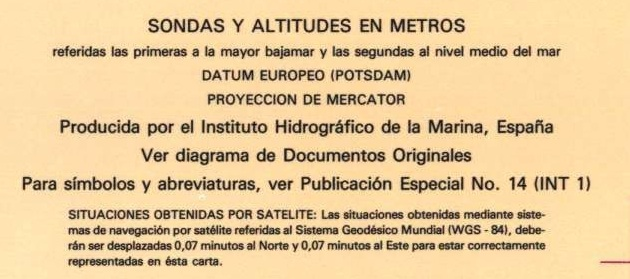
\includegraphics[width=\textwidth]{datum-europeo}\\
%\caption{Tarjeta de una carta referida al datum europeo.}
%\label{fg:datum-europeo}
%\end{center}
%\end{figure}

\begin{ejemplo}
En la tarjeta de de una carta referida al datum europeo %(figura\ref{fg:datum-europeo})
figura el siguiente párrafo: 
\begin{quotation}\noindent\itshape\color{darkblue}
SITUACIONES OBTENIDAS POR SATÉLITE: Las situaciones obtenidas mediante sistemas 
de navegación por satélite referidas al Sistema Geodésico Mundial (WGS-84) deberán ser 
desplazadas 0,07 minutos al Norte y 0,07 minutos al Este para estar correctamente representadas en esta carta. 
\end{quotation}
Si se ha obtenido una situación por satélite referida al sistema WGS84 igual a 37º44,02’\,N
0º42,35’\,W, la trazaremos en la carta como 37º44,09’\,N 0º42,28’\,W. En una carta de punto mayor
la diferencia es imperceptible (0,4\,mm, aproximadamente, para una escala de 1:300\,000), pero si usamos cartas de 
punto mayor es muy importante hacer la correción del datum. Así, por ejemplo, la corrección de 0,07’ 
de latitud (129,6\,m) equivale a 2,6\,mm en una carta de escala 1:50\,000, y a 8,6\,mm en un portulano de escala
 1:15\,000.
\end{ejemplo}

Como vemos en el ejemplo anterior, cuando se quiere obtener situaciones precisas con 
sistemas de navegación por satélite es necesario tener en cuenta el datum de la carta y 
hacer las correcciones necesarias. 

\subsubsection{Datum vertical }

\index{datum!vertical}
\index{bajamar escorada}

El \emph{datum vertical} es la referencia que se usa para medir las elevaciones (en tierra) y las 
sondas (en la mar). En las cartas españolas las elevaciones se miden siempre en metros 
sobre el nivel medio del mar, y las sondas también en metros, referidas a la bajamar 
escorada (ver capítulo \ref{ch:mareas}). 

En las cartas inglesas y norteamericanas antiguas se miden las elevaciones en pies (ft),%
%\footnote{\emph{Feet}.} 
 y las sondas en brazas (fm)%
%\footnote{\emph{Fathoms}.}
 y pies, aunque en las cartas modernas estas magnitudes se 
miden en metros. En estas cartas las sondas se refieren al nivel medio de la bajamar de 
mareas vivas. 

%--------------------------------------------------------------
\subsection{Rosa náutica y declinación magnética}

\index{rosa}
\index{rosa!náutica}
\index{rosa!de los vientos|see rosa náutica}
\index{declinación!magnética}
\index{declinación!variación anual}

Una rosa náutica es una figura consistente en dos círculos graduados concéntricos que indican 
rumbos verdaderos y magnéticos, respectivamente (figura \ref{fg:rosa}). 
En la dirección que señala el Norte magnético se indica el valor de la declinación magnética 
para un año determinado, y el valor de la variación anual de la misma. 
Cuando la declinación magnética varía significativamente de una parte a otra de la 
carta, su valor se indica mediante distintas rosas o con rótulos adicionales. En estos casos 
hay que emplear el valor de la declinación indicado en la rosa o rótulo más próximo a la 
zona de la carta con la que se esté trabajando. 

\begin{figure}[htbp]
\begin{center}
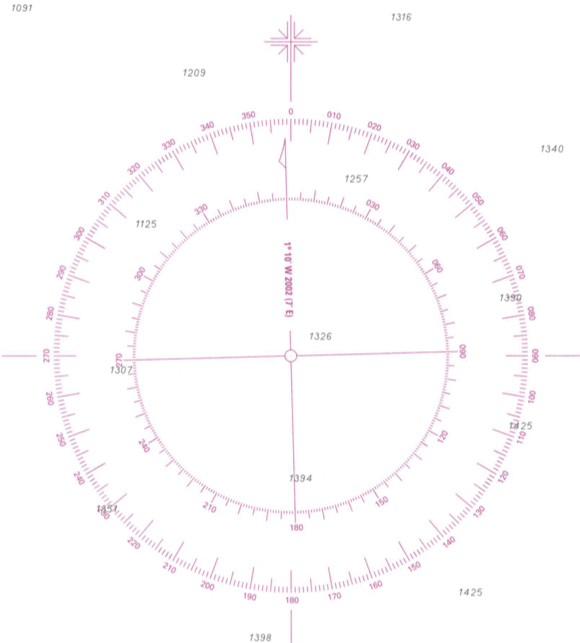
\includegraphics[scale=0.5]{rosa}\\
\caption{Rosa náutica.}
\label{fg:rosa}
\end{center}
\end{figure}

\begin{ejemplo}
El valor de la declinación magnética en la zona de la carta donde se encuentra la rosa 
de la figura \ref{fg:rosa} es de 1º10’\,W en 2002. La variación anual es de 7’\,E. 
Por tanto, en 2009 la declinación será:
\[
\begin{array}{lcll}
  \mbox{Valor en 2002} & =  & -1º \, 10' \: \mathrm{(W)} \\
  \mbox{Variación}     & =  & +1º \, 10' \: \mathrm{(E)} & (\mbox{7 años} \times 10' = 70' )\\
%  \cline{3-5}\\
\mbox{Valor en 2009}  &  = & \hspace{1\plus}0º \, 00’ \: \mathrm{(W)} &  
\end{array}
\]
\end{ejemplo}

%--------------------------------------------------------------
\subsection{Detalles de las cartas}

Las figuras \ref{fg:cedeira} y \ref{fg:471a} muestran sendos fragmentos de dos cartas náuticas: 
el aproche de la ría de Cedeira incluido en la carta nº~930, y la carta de navegación costera 
nº~471A del IHM. En ambas se pueden apreciar la mayoría de los detalles que suelen aparecer en las 
cartas náuticas. 

\begin{figure}[htbpp]
\begin{center}
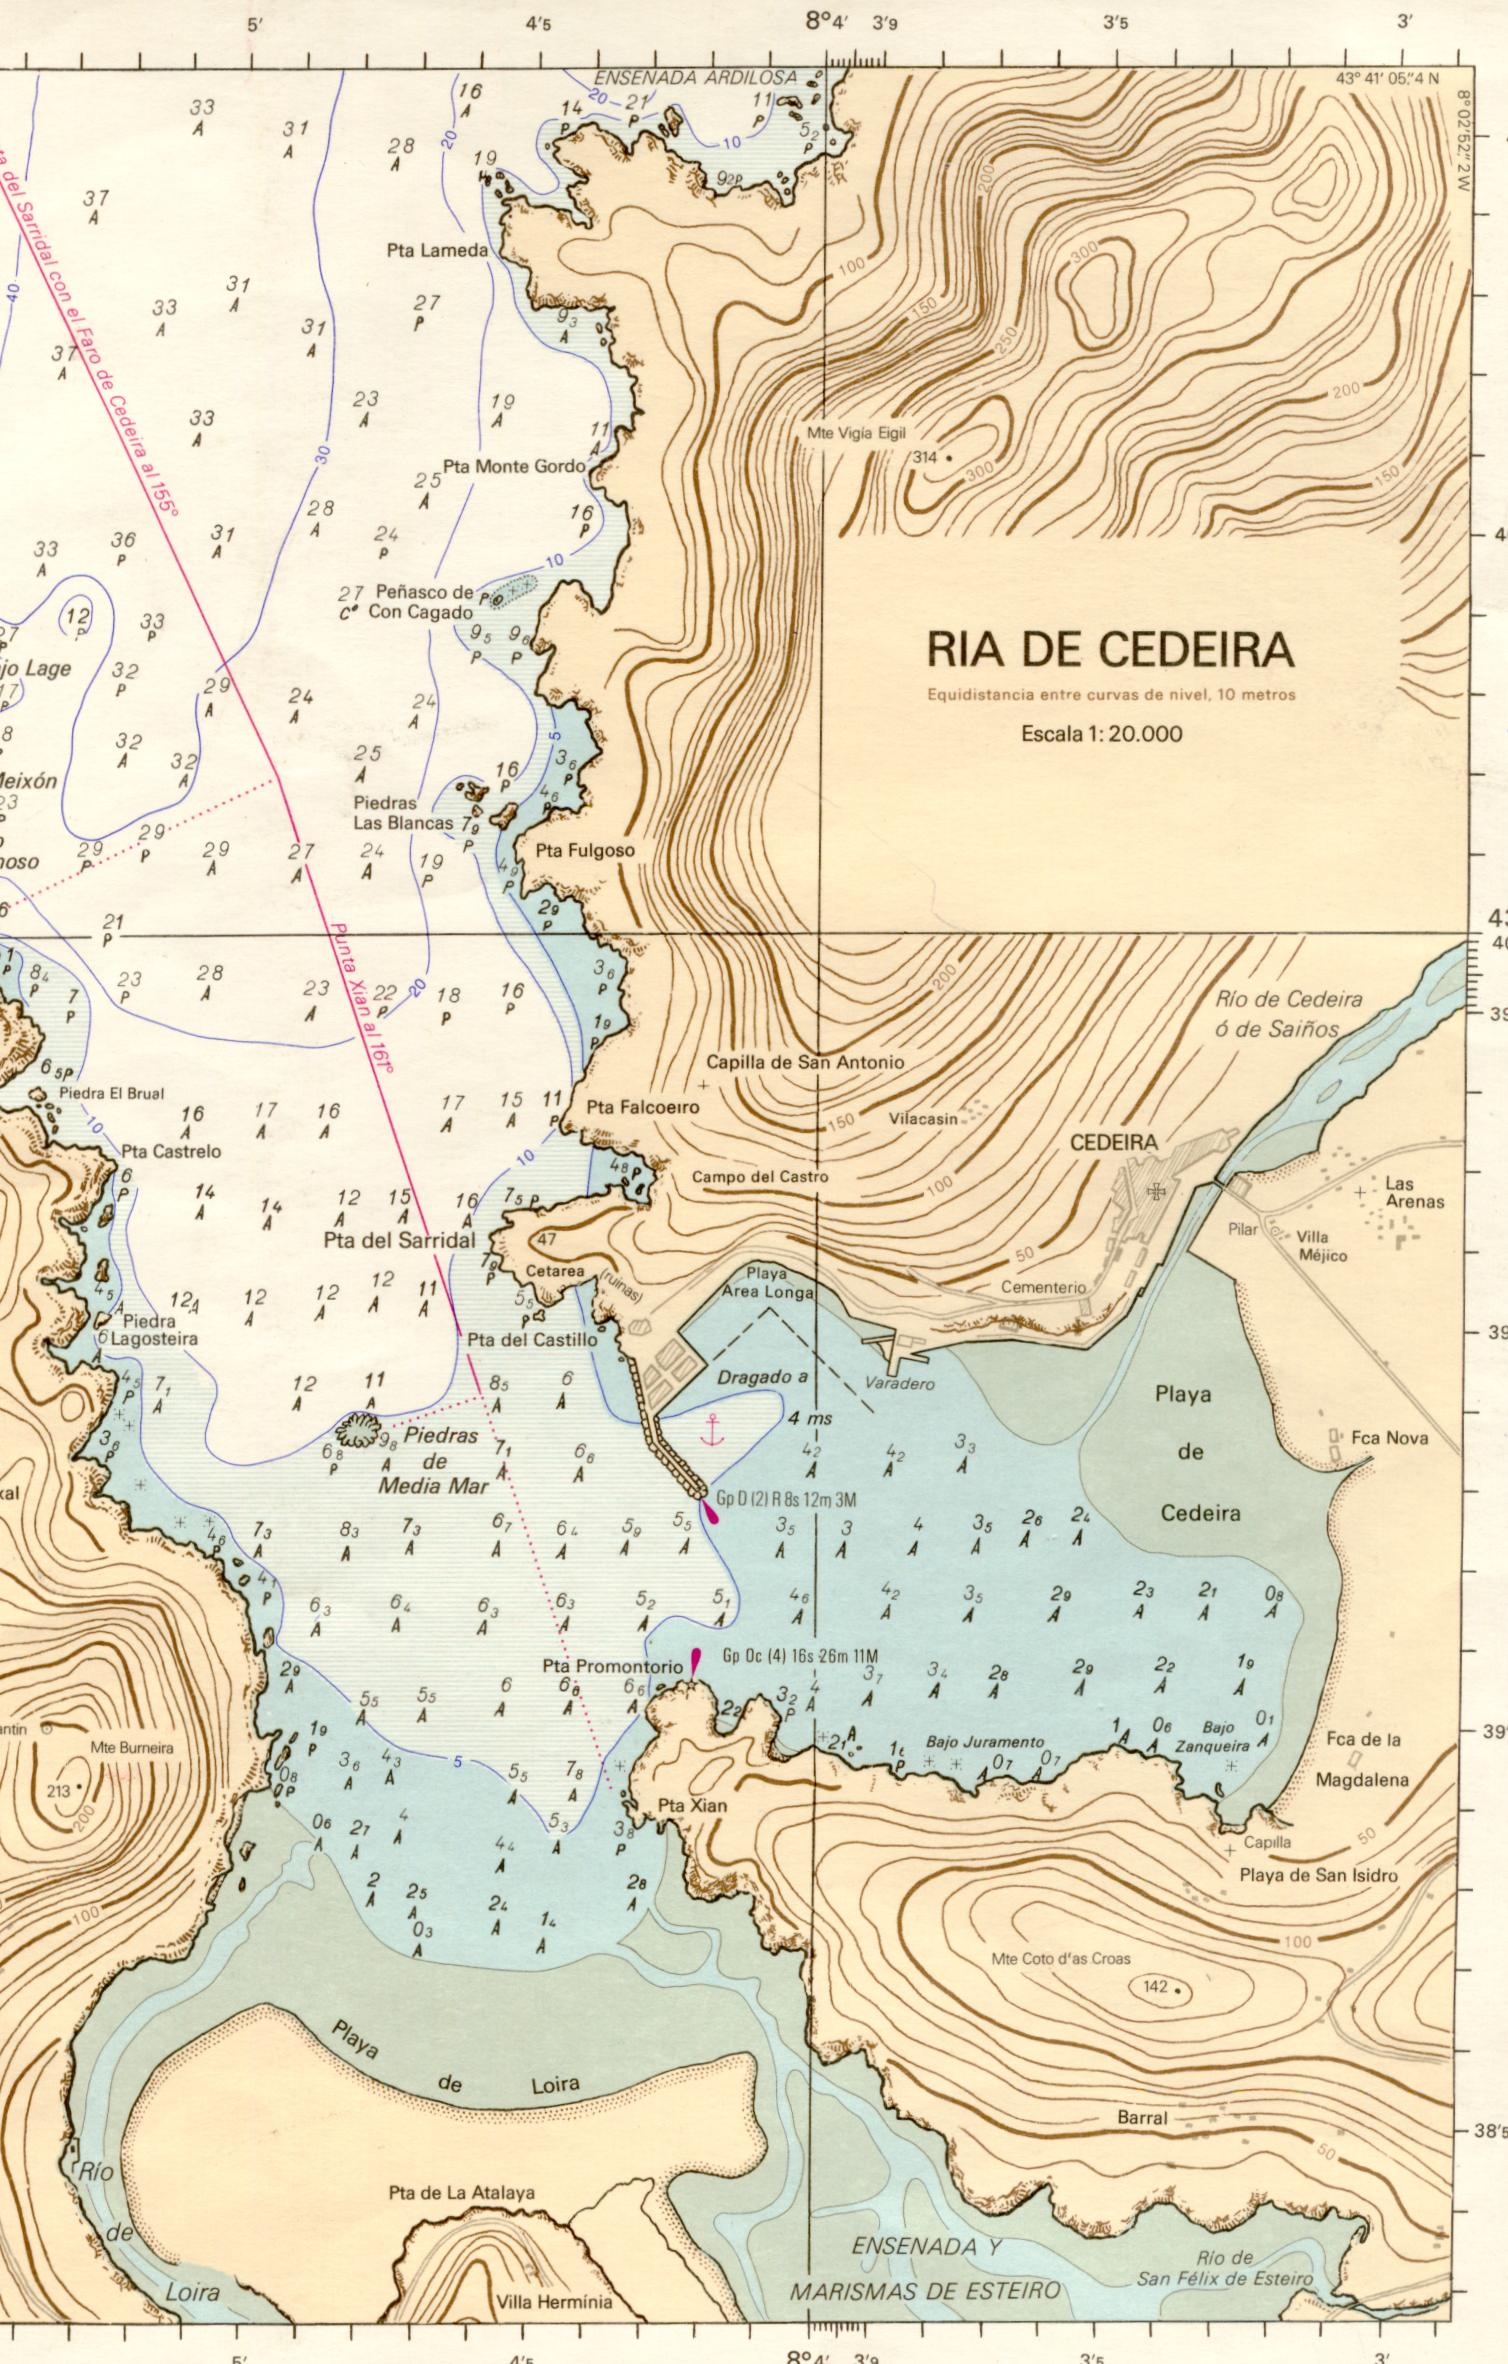
\includegraphics[width=\textwidth]{cedeira}\\
\caption{Aproche de la ría de Cedeira (cartucho de la carta nº930 del IHM).}
\label{fg:cedeira}
\end{center}
\end{figure}

\begin{figure}[htbpp]
\begin{center}
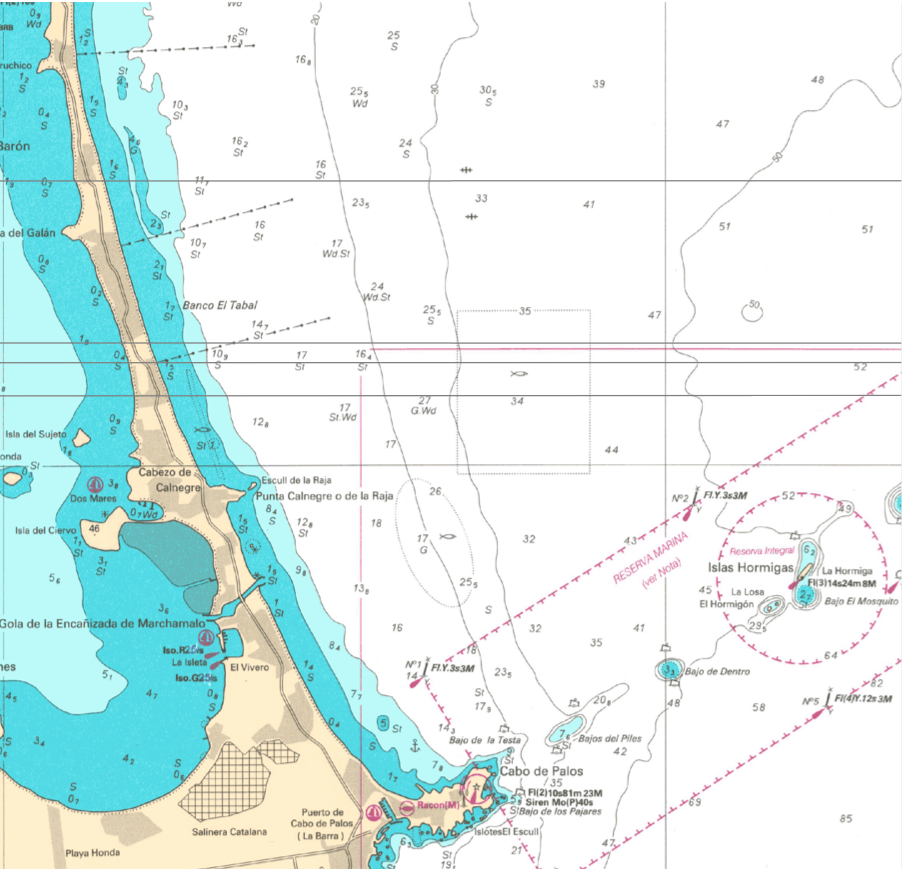
\includegraphics[width=\textwidth]{cabopalos}\\
\caption{Fragmento de la carta 471A del IHM.}
\label{fg:471a}
\end{center}
\end{figure}


\subsubsection{Signos y abreviaturas }

La publicación especial nº~14 (INT1) del Instituto Hidrográfico de la Marina contiene 
todos los símbolos, abreviaturas y términos usados en las cartas oficiales españolas. Los 
símbolos son los recomendados por la Organización Hidrográfica Internacional (OHI), 
aunque en algunos casos las cartas españolas de una cierta antigüedad utilizan símbolos 
nacionales distintos de aquéllos. Estos símbolos nacionales se explican también en la 
publicación nº 14. 

\subsubsection{Profundidad y naturaleza del fondo}

La profundidad medida en distintos puntos de la carta se indica mediante \emph{sondas}. 
Las sondas se refieren al datum vertical de la carta (la bajamar escorada en las cartas 
españolas), y se representan mediante números que indican la profundidad en metros y, en su 
caso, en decímetros, en el punto donde se encuentran. La cifra que indica 
los decímetros se escribe como un subíndice. Las sondas que se encuentran 
fuera de posición, es decir las que se refieren a un punto cercano a aquél 
donde se encuentran, se escriben entre paréntesis. La sondas medidas con 
precisión se escriben en cursiva, mientras que las dudosas o las 
obtenidas de otros documentos menos fiables se escriben con números rectos 
(figura \ref{fg:sondas}). Las sondas negativas corresponden a 
puntos que velan en la bajamar escorada, aunque pueden quedar sumergidos 
al subir la marea (capítulo \ref{ch:mareas}), se escriben subrayadas. 

\begin{figure}[htbp]
\begin{center}
\begin{tabular}{>{\itshape\color{blue}}m{1cm} >{\upshape}m{6cm}}\toprule
{35 \newline S} & Sonda de 35 m con fondo de arena.     \\ \addlinespace[1ex]
{12\textsubscript{7} \newline St} & Sonda de 12,7\,m con fondo de piedra.\\ \addlinespace[1ex]
{(8\textsubscript{2}) } &  Sonda de 8,2\,m en un punto cercano. \\ \addlinespace[1ex]
{\upshape 15} & Sonda de 15\,m aproximada.\\ \addlinespace[1ex]
{\underline{1\textsubscript8} } & sonda negativa de 1,8\,m.\\ \addlinespace[1ex]
\bottomrule
\end{tabular}
\caption{Ejemplos de sondas.}
\label{fg:sondas}
\end{center}
\end{figure}

\begin{ejemplo}
En un punto en donde la carta marca \underline{\itshape1\textsubscript{8}} 
la profundidad del agua es igual a 0,7\,m cuando la altura de la marea es de 2,5\,m. 
Cuando la altura de la marea es menor que 1,8\,m el punto vela
 (es decir, está fuera del agua). 
\end{ejemplo}

Las sondas suelen ir acompañadas de una abreviatura, situada debajo de ellas, que
indica la naturaleza del fondo. La figura \ref{fg:fondo} muestra algunas de las 
abreviaturas más comunes en español y en inglés. 
En las cartas españolas modernas figura siempre la abreviatura 
en inglés, de acuerdo con las normas internacionales.

\begin{figure}[htbp]
\begin{center}
\begin{tabular}{>{\itshape\color{blue}}c 
                >{\itshape\color{blue}}c
                >{\upshape}l}\toprule
A & S & Arena (\emph{sand}) \\
F & M & Fango (\emph{mud}) \\
P & St & Piedra (\emph{stone}) \\
C\textsuperscript{o} & G & Cascajo (\emph{gravel}) \\
G\textsuperscript{o} & P & Guijarros (\emph{pebbles}) \\
R & R & Roca (\emph{rock}) \\
Alg & Wd & Algas (\emph{weed}) \\
\bottomrule
\end{tabular}
\caption{Tipos de fondos.}
\label{fg:fondo}
\end{center}
\end{figure}


Los \emph{veriles} o \emph{líneas isobáticas} son líneas que unen todos los puntos 
que tienen una misma profundidad (por ejemplo, 10\,m, 20\,m o 100\,m). Las zonas 
delimitadas por los veriles de menor profundidad, dependiendo de la escala y del 
tipo de carta, se colorean con distintos tonos de azul. La zona cercana a la
costa que queda al descubierto en la bajamar se colorea de verde claro. 

\subsubsection{Peligros}
 
Los distintos peligros que se encuentran en la mar, como piedras, bajos, 
restos de naufragios, etc. se indican en las cartas mediante
diversos signos, los más importantes de los cuales se muestran en la figura \ref{fg:peligros}. 

\begin{figure}[htbp]
\begin{center}
\begin{tabular}{m{8mm}
                >{\itshape\color{blue}}m{6mm}
                >{\upshape}m{5cm}}
                \toprule
\
\centering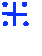
\includegraphics[scale=0.75]{piedra}  && Roca a flor de agua.  \\
\centering
\includegraphics[scale=0.75]{piedra-sumergida} && Roca cubierta peligrosa. \\
\centering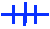
\includegraphics{pecio} &Wk & Naufragio \\
\bottomrule
\end{tabular}
\caption{Símbolos de peligros.}
\label{fg:peligros}
\end{center}
\end{figure}

\subsubsection{Marcas y luces }

Las cartas muestran de forma detallada la situación de las marcas terrestres útiles para la
navegación, y de las boyas, balizas, luces y otras ayudas. Las luces se indican con una
marca púrpura, junto con sus características luminosas (figura \ref{fg:luces}).
 Los sectores visibles o de distintos colores, en su caso, se indican
también gráficamente en la carta. También se indica la altura de la luz sobre el nivel medio
del mar y su alcance en millas. Todos estos datos se encuentran igualmente en el
 \emph{Libro de Faros}, donde debe acudirse siempre para una referencia más completa y exacta. 


\begin{figure}[htbp]
\begin{center}
\begin{tabular}{>{\color{blue}}m{12mm}
                >{\bfseries\color{blue}}m{10mm}
                >{\upshape}l}\toprule
 
\includegraphics{faro} &
 & Luz, faro \\
 F.  & F & Fija (\emph{fixed}). \\
 Oc. & Oc & Ocultaciones (\emph{occulting}) \\
 D   & Fl & Destellos (\emph{flaring}) \\
 Gp. D. & Fl(3) & Grupos de destellos \\
 Ct.    & Q     & Centelleos (\emph{quick}) \\
 B      & W     & Blanca (\emph{white}) \\
 R      & R     & Roja (\emph{red}) \\
 V      & G     & Verde (\emph{green}) \\
\bottomrule
\end{tabular}
\caption{Símbolos y abreviaturas de luces y faros.}
\label{fg:luces}
\end{center}
\end{figure}

\subsection{Puesta al día de las cartas }

La información que contienen las cartas sólo es exacta en la fecha de su última actualización, 
que en el momento de su adquisición está escrita en el margen inferior (figura \ref{fg:id-carta}). 
Para mantenerlas al día es preciso actualizarlas con las correcciones que se publican cada 
semana en los \emph{Avisos a los navegantes}, editados por el Instituto Hidrográfico de la 
Marina. 

%===================================
\section{Trabajo sobre la carta}

\subsection{Instrumentos}
 
Los trabajos gráficos sobre la carta se efectúan con lápiz, compás de puntas o compás 
ordinario (con mina de lápiz), transportador y regla. También hay 
instrumentos que combinan un transportador y una regla, de forma rectangular o triangular.
Estos instrumentos son más fáciles de utilizar que los transportadores tradicionales 
en el reducido espacio de la mesa de cartas. 

\subsection{Situaciones}
 
 \begin{figure}[htbp]
\begin{center}
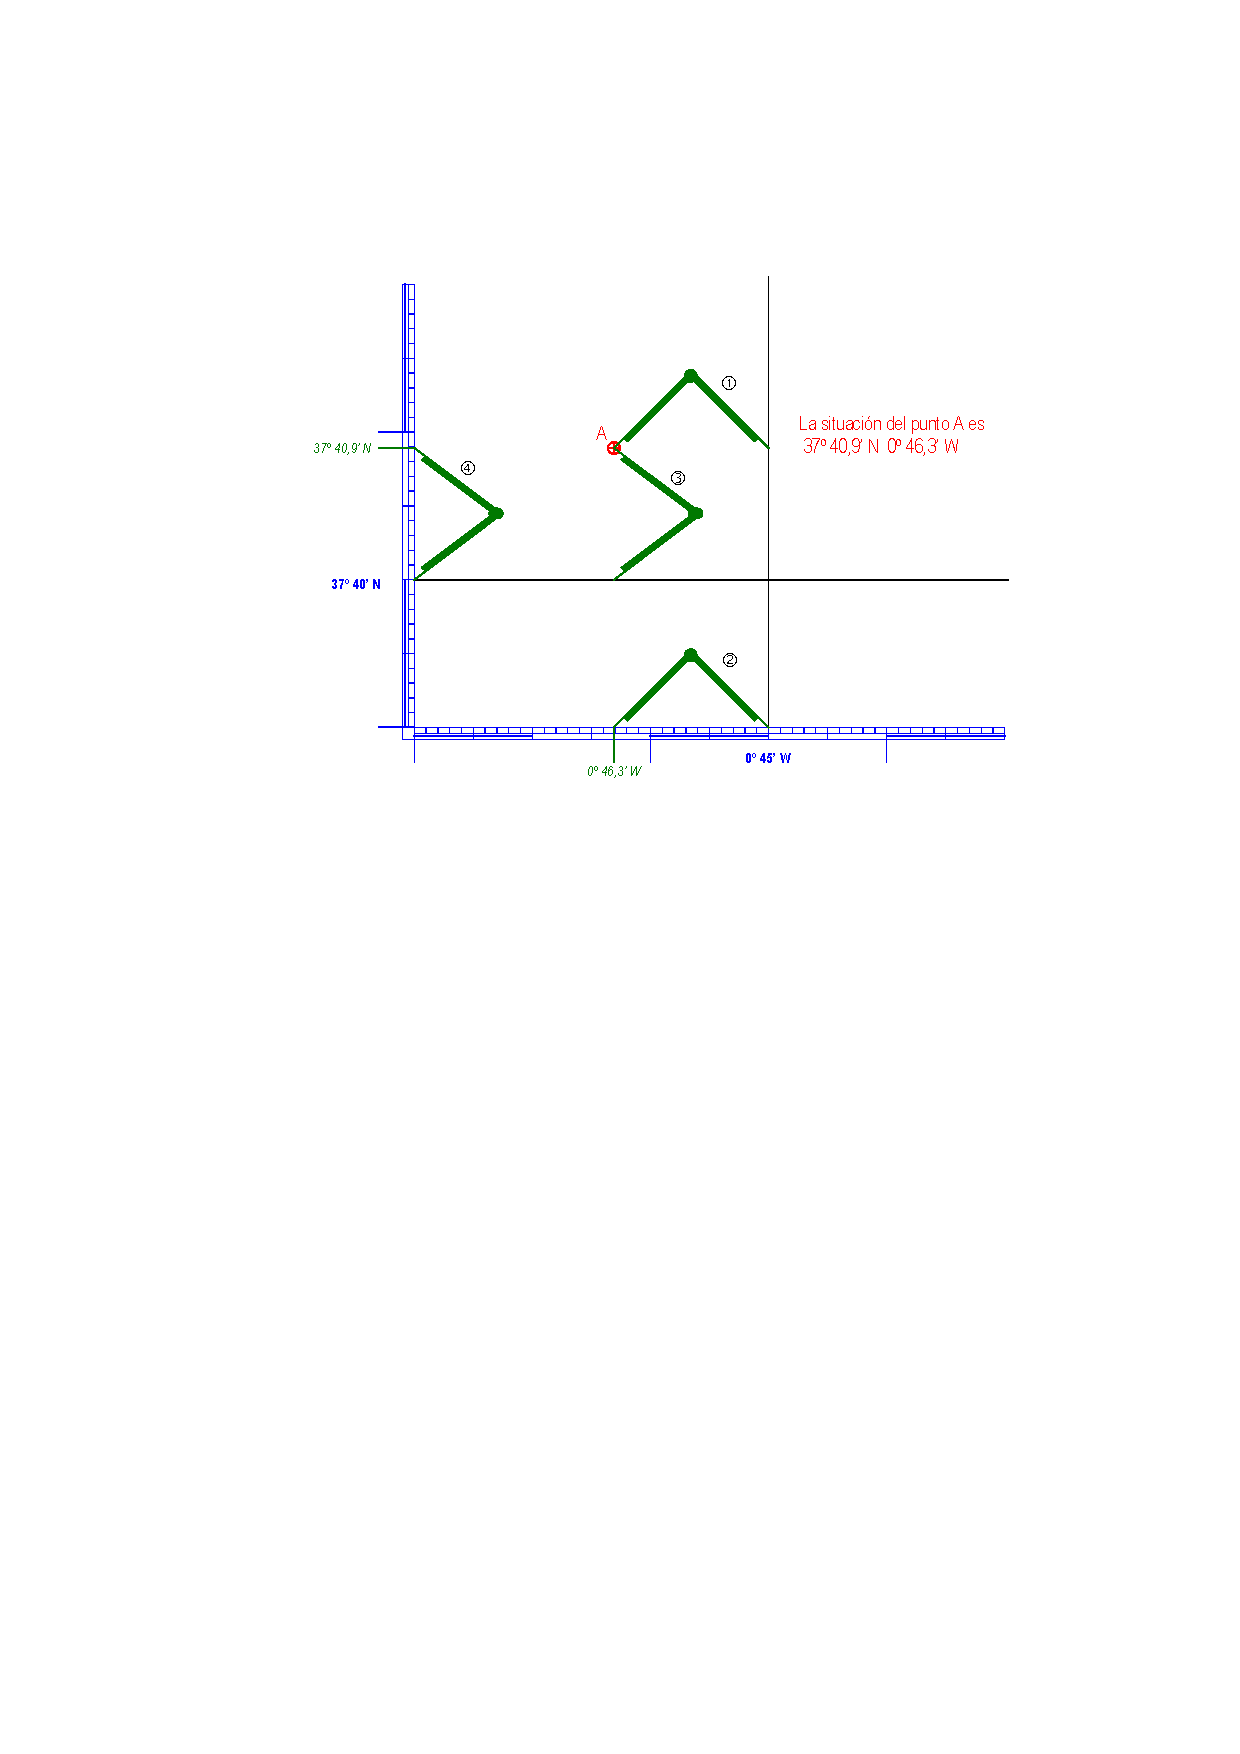
\includegraphics{carta-coordenadas}
\caption{Forma de hallar las coordenadas de un punto.}
\label{fg:carta-coordenadas}
\end{center}
\end{figure}

\subsubsection{Obtener las coordenadas de un punto de la carta}

Para obtener las coordenadas de un punto se utiliza normalmente un compás, una de 
cuyas puntas se coloca en el punto (figura \ref{fg:carta-coordenadas}, 1). 
Con la otra punta se tangentea el paralelo más próximo, y manteniendo la abertura 
del compás se mide la latitud en la escala de latitudes de la carta (2). 
Para la longitud se opera de forma semejante (3 y 4). 


\begin{figure}[htbp]
\begin{center}
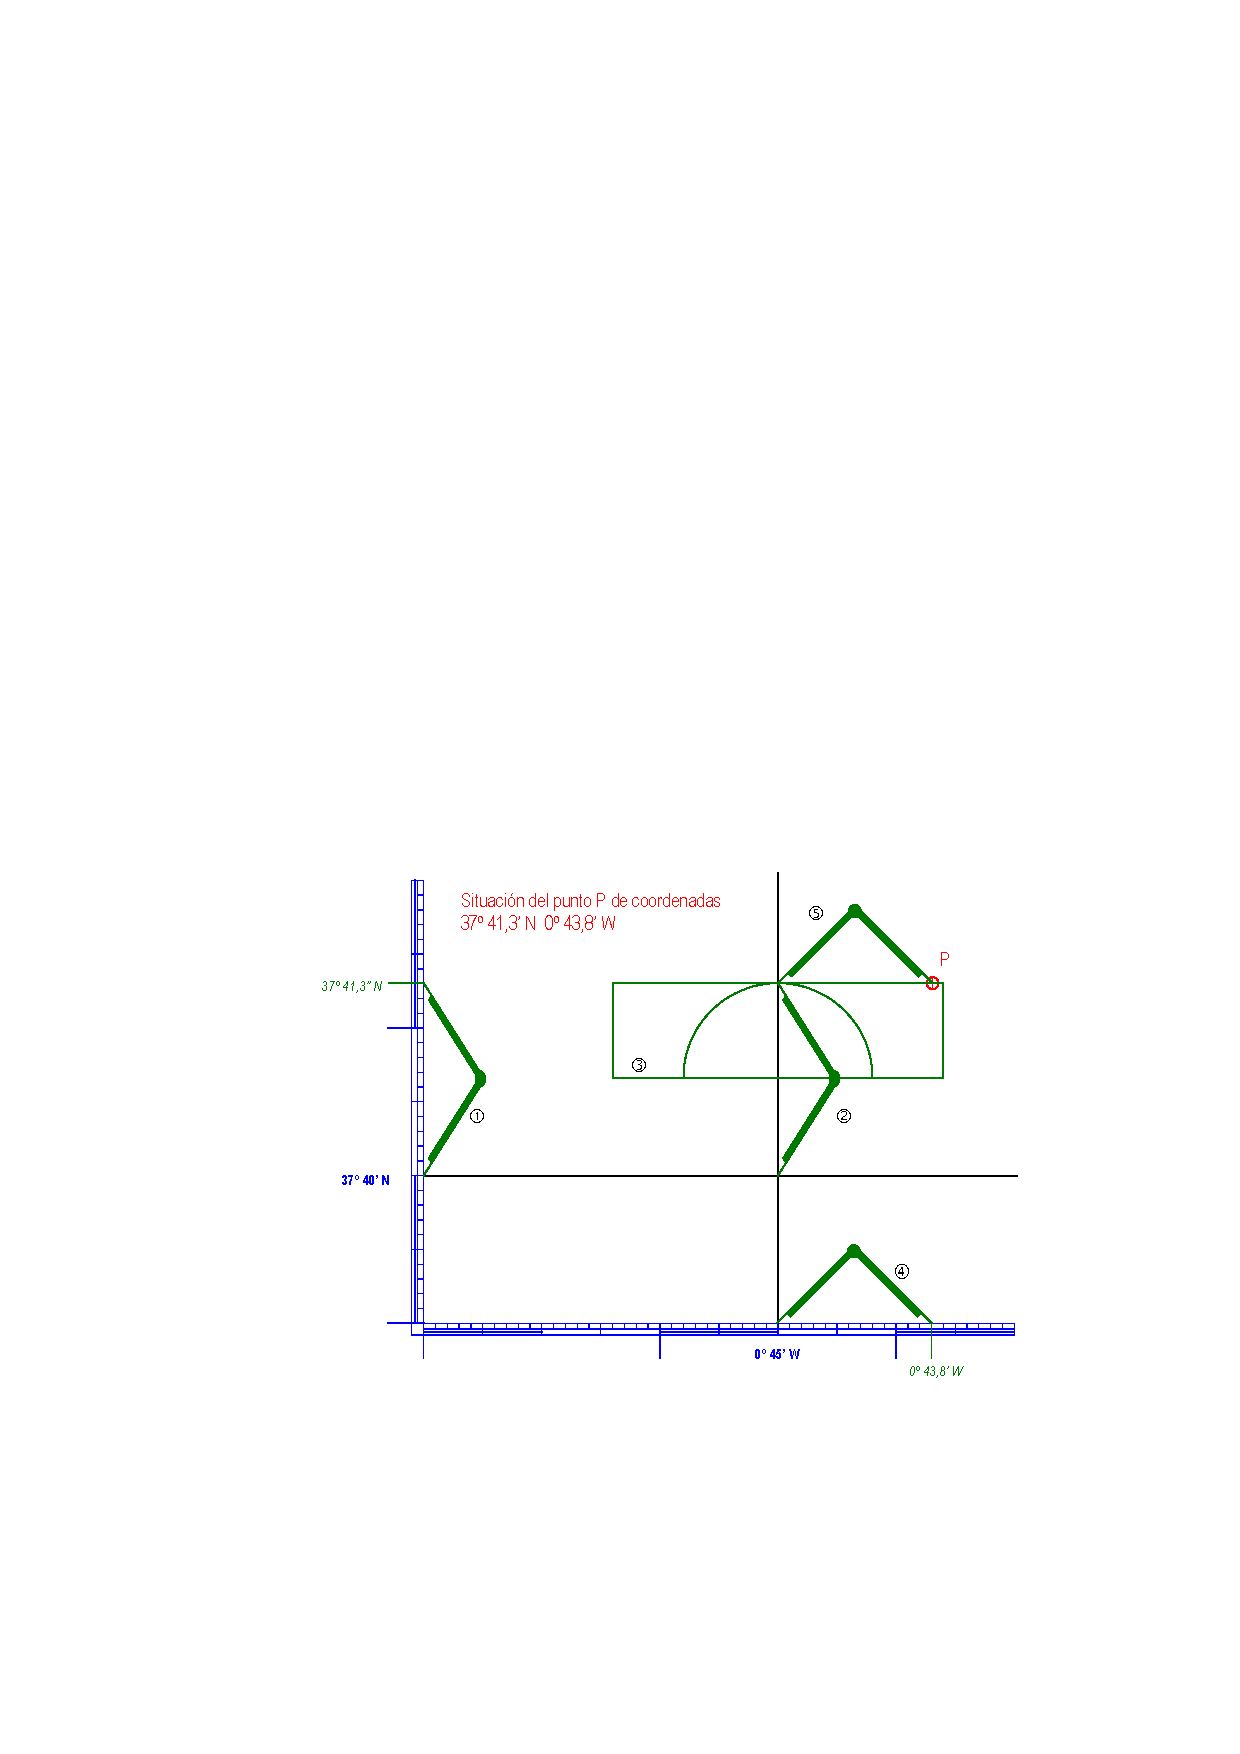
\includegraphics{carta-situacion}
\caption{Forma de situar un punto dadas sus coordenadas.}
\label{fg:carta-situacion}
\end{center}
\end{figure}

\subsubsection{Situar un punto dadas sus coordenadas}

Para situar un punto en la carta, se coloca una punta del compás en la marca 
correspondiente a la latitud en la escala de latitudes, y la otra punta en el paralelo 
más cercano en la misma escala (figura \ref{fg:carta-situacion}, 1). La abertura del compás se traslada 
al meridiano más cercano al punto, a partir del mismo paralelo (2), y se marca el 
punto correspondiente. Se coloca el transportador de forma que su borde superior 
pase por el punto marcado y esté perpendicular al meridiano, y sobre este borde 
se lleva la abertura de compás que previamente se ha tomado sobre la escala de longitudes,
entre el meridiano anterior y la longitud buscada (4 y 5).

\begin{figure}[htbp]
\begin{center}
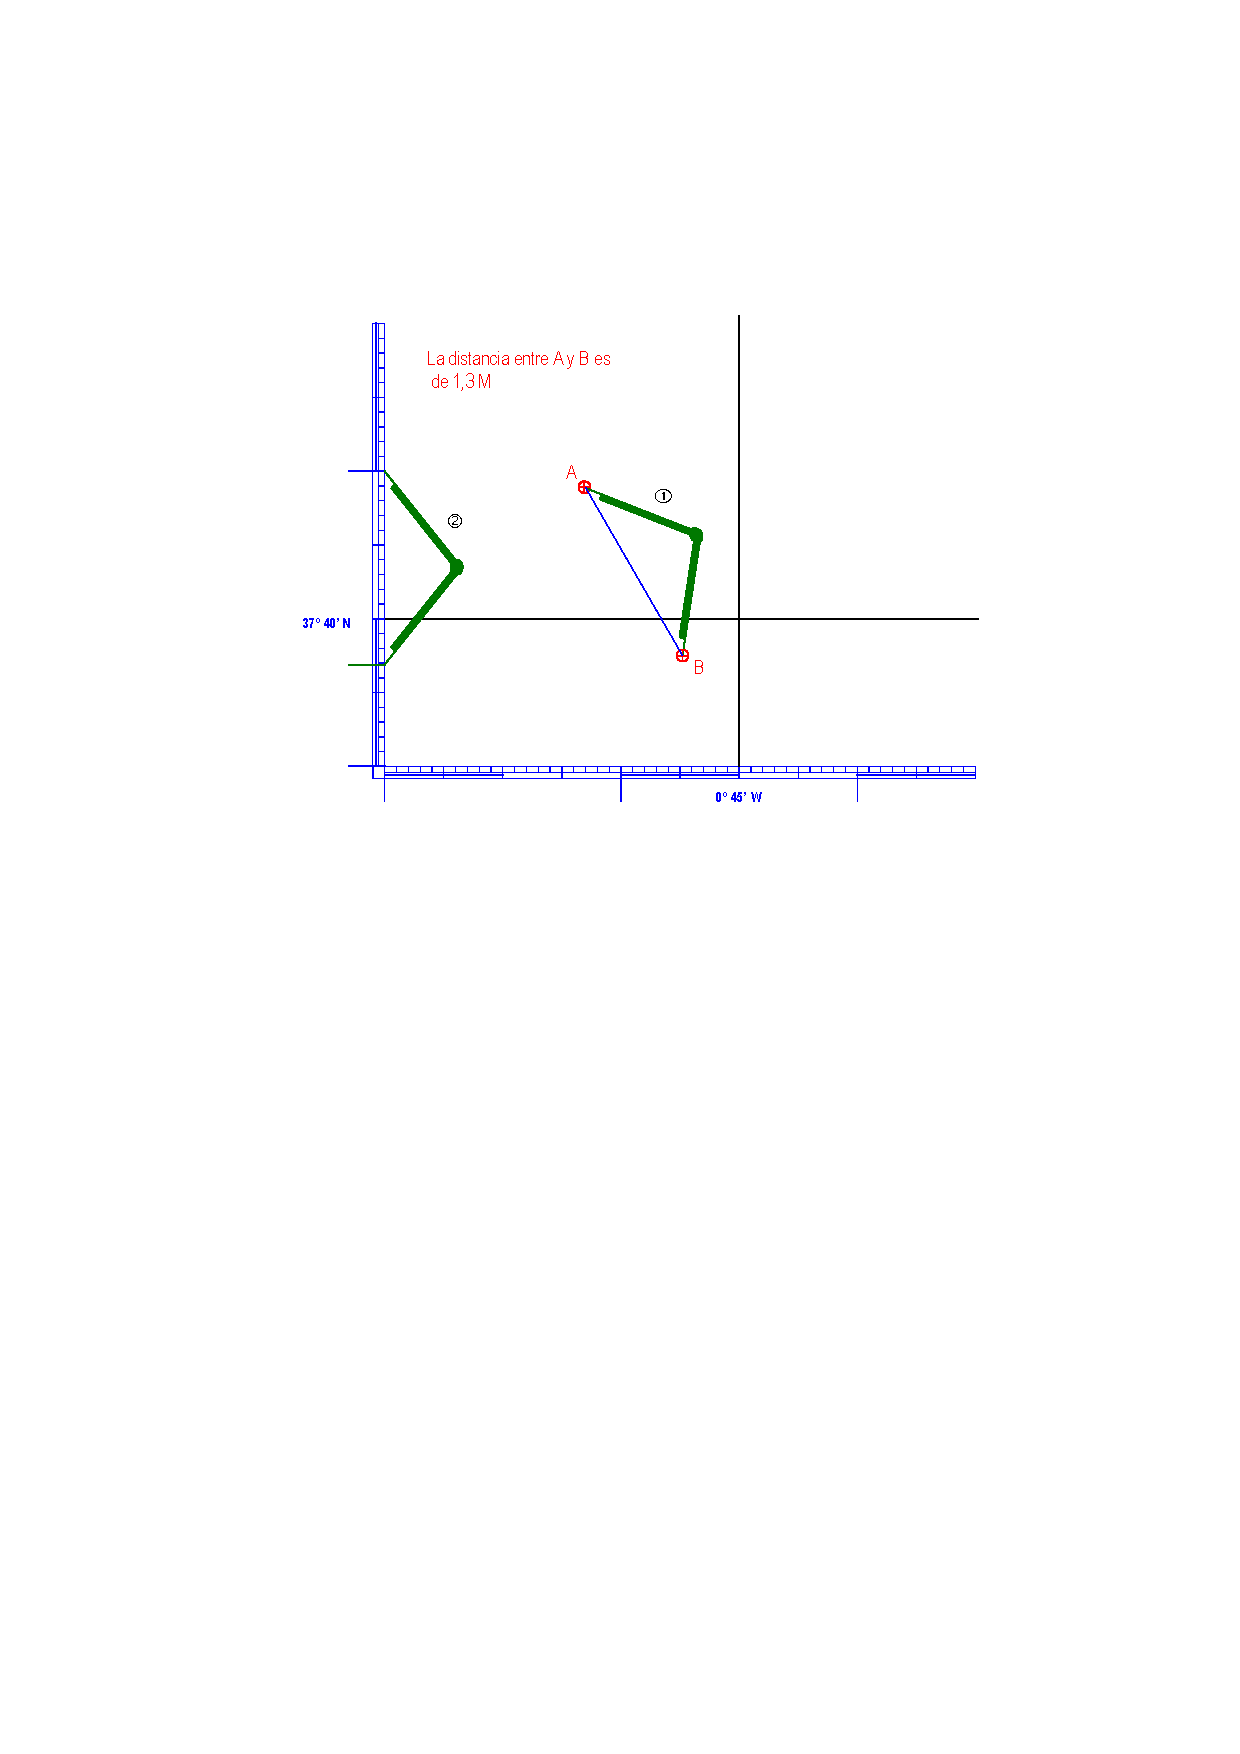
\includegraphics{carta-distancia}
\caption{Medida de la distancia entre dos puntos.}
\label{fg:carta-distancia}
\end{center}
\end{figure}


\subsubsection{Distancia entre dos puntos}

Para medir la distancia entre dos puntos se coloca cada una de las puntas del compás 
sobre uno de los puntos (figura \ref{fg:carta-distancia}, 1), y se lleva 
la abertura correspondiente a la escala 
de latitudes más cercana (2). La distancia en millas entre los dos puntos es igual al 
intervalo de latitud en minutos que corresponde a la apertura del compás. 
Hay que tener cuidado de que la parte de la escala que se utilice esté aproximadamente 
a la misma latitud que los puntos cuya distancia se desea medir, sobre todo si la 
carta abarca una gran diferencia de latitudes. En este caso, al variar de forma apreciable la 
escala con la latitud podríamos obtener un valor de la distancia falseado. 
Para situar un punto a una distancia dada de otro se procede de forma inversa, 
midiendo primero la distancia sobre la escala de longitudes y llevándola después sobre la 
línea donde se desea situar el punto. 

\begin{figure}[htbp]
\begin{center}
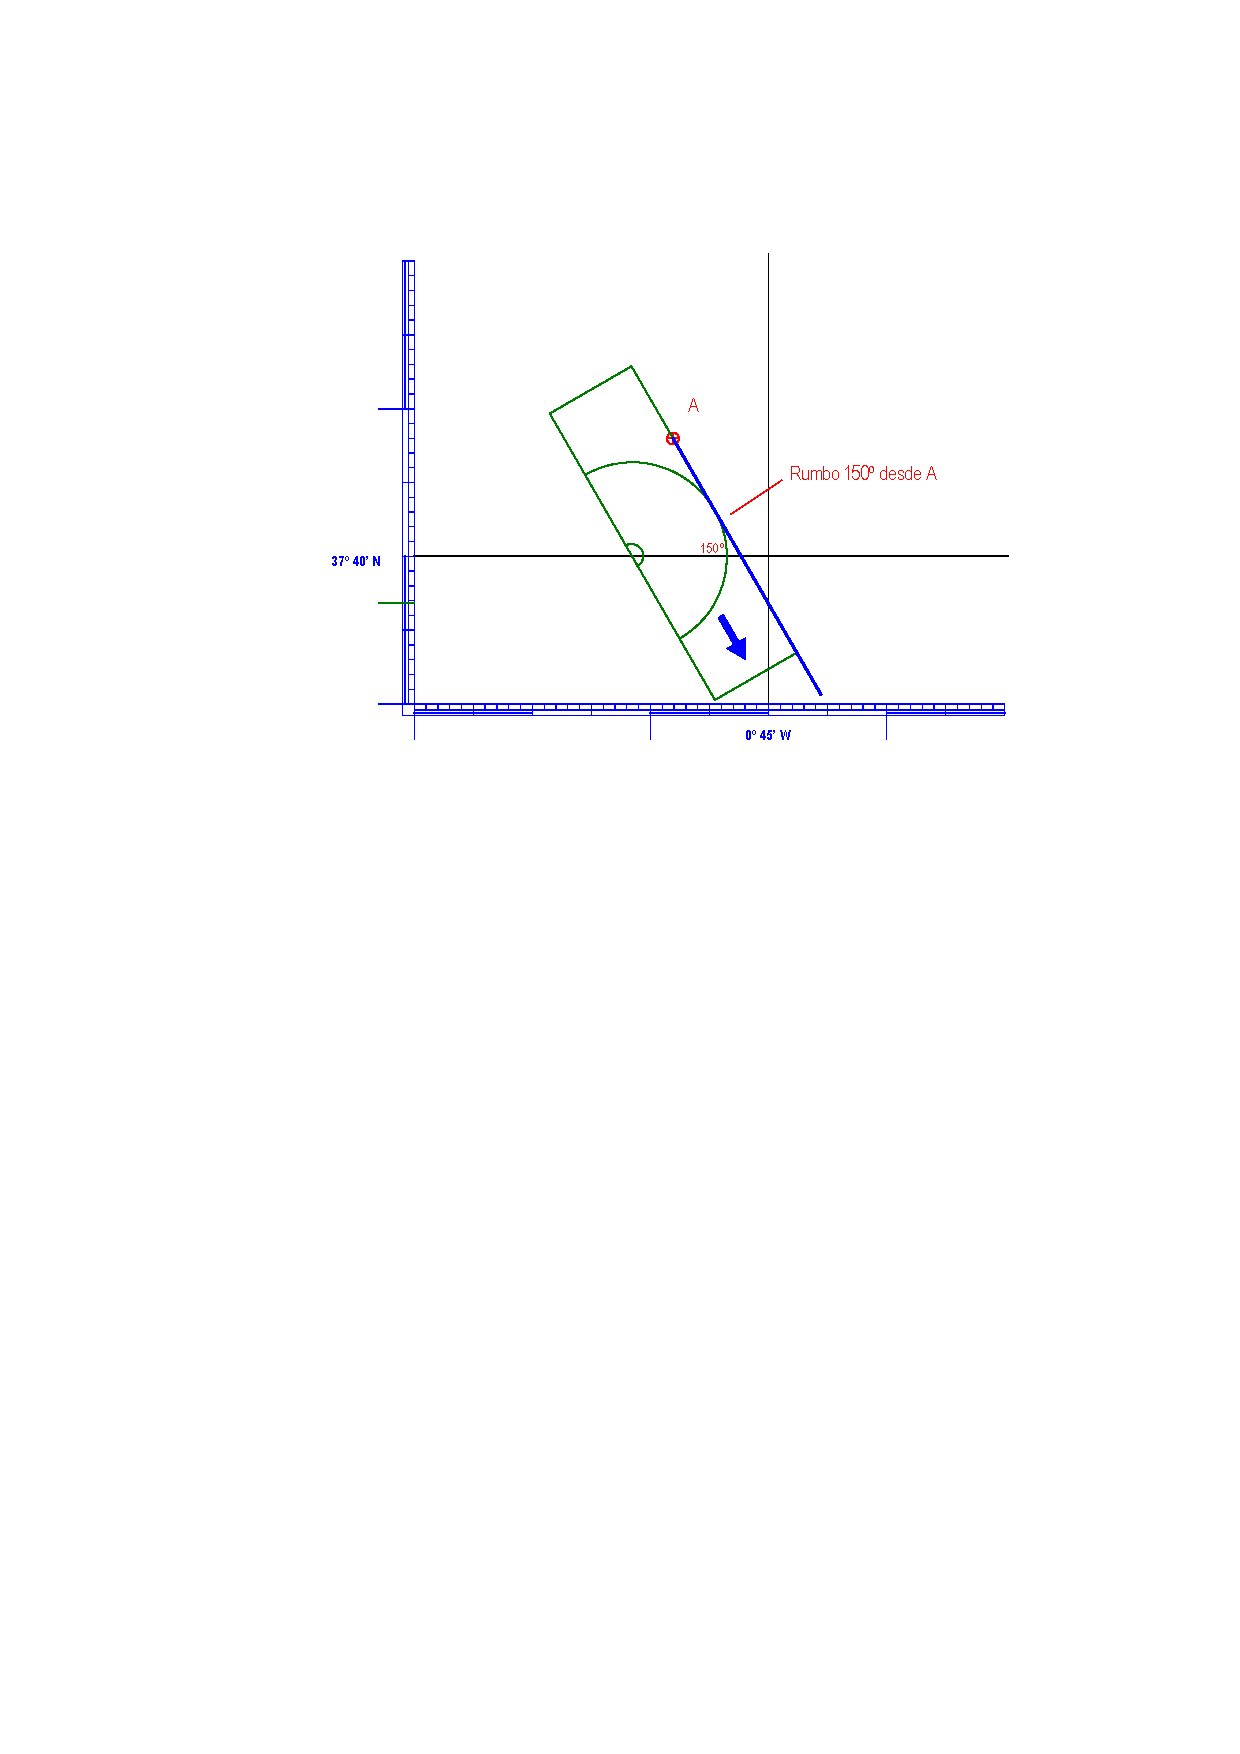
\includegraphics{carta-rumbo}
\caption{Trazado de rumbos y demoras.}
\label{fg:carta-rumbo}
\end{center}
\end{figure}

\subsubsection{Rumbos y demoras}

Las líneas que forman un ángulo constante con la dirección Norte (loxodrómicas), como 
son los rumbos y demoras, se representan en la carta mediante rectas, como ya hemos 
visto. Para trazar la línea correspondiente a un rumbo o una demora dada pasando por un 
punto determinado se utiliza la regla-transportador, situando el centro de la escala de 
ángulos en un meridiano o paralelo, orientando el instrumento de forma que se lea la gra- 
duación correspondiente al rumbo sobre dicho meridiano o paralelo, y situando uno de los 
bordes sobre el punto (figura \ref{fg:carta-rumbo}). 
En cualquier caso, es necesario familiarizarse con el 
instrumento que se utilice, y practicar en la mesa de cartas del barco para efectuar el tra- 
zado con soltura. 

Para medir el rumbo entre dos puntos se procede de forma inversa: se coloca la regla- 
transportador de manera que su centro se sitúe sobre un meridiano o paralelo y su borde 
pase por ambos puntos. El rumbo se lee directamente sobre la escala del transportador. 
Como antes, es necesario practicar para efectuar esta operación con soltura. 

%===================================
\section{Cartas electrónicas}

Las cartas electrónicas contienen una información similar a las cartas tradicionales 
impresas en papel, pero están almacenadas en forma digital en un soporte electrónico o 
magnético adecuado para su lectura e interpretación por un computador. Este computador puede 
ser de tipo general (por ejemplo, un computador personal) o estar empotrado en un 
instrumento de navegación, como una pantalla de radar o un navegador por satélite. En todos 
los casos se usan diferentes formatos para la representación de los datos de las cartas, 
algunos de los cuales son cerrados, es decir sólo se pueden leer con los programas o ins- 
trumentos fabricados por una compañía determinada. Siempre que sea posible se deben 
preferir las cartas almacenadas en formatos abiertos, que se pueden leer con programas e 
instrumentos de distintos fabricantes. 

Hay dos tipos de cartas digitales: las \emph{cartas escaneadas} y las 
\emph{cartas vectoriales}. Cada uno de estos tipos tiene sus ventajas e inconvenientes, 
aunque en general las cartas vectoriales son más precisas y fáciles de usar. 

\subsection{Tipos de cartas electrónicas}

\subsubsection{Cartas escaneadas}

Las cartas escaneadas son reproducciones directas de las cartas de papel realizadas 
mediante un escáner o un aparato similar, que produce una imagen formada por una cua- 
drícula de puntos (\emph{raster}). Su principal ventaja es que reproducen exactamente las cartas 
oficiales, por lo que en general se puede confiar en ellas, siempre que se mantengan al 
día. Otra ventaja es que son relativamente fáciles de construir, y que si se almacenan en 
un formato abierto se pueden ver en un computador mediante programas corrientes. 
El principal inconveniente de las cartas escaneadas es que cuando se amplían no se 
consigue mayor detalle, e incluso se hacen visibles los puntos de la cuadrícula, perdién- 
dose calidad de imagen. 

\subsubsection{Cartas vectoriales}

Las cartas vectoriales, de construcción más elaborada, representan cada elemento de la 
carta (línea de costa, peligros, balizas, faros, etc.) mediante una estructura de datos 
(vector) que contiene información sobre su situación, nombre, representación gráfica, etc. Los 
puntos que forman la imagen se forman sobre la marcha al ver la carta en un visor ade- 
cuado. De esta manera, al ampliar la carta no se pierde resolución, ya que los detalles que 
aparecen se vuelven a dibujar cada vez. Además, casi todos los visores permiten seleccio- 
nar los detalles que se ven, que se agrupan en distintas capas, por ejemplo 
(figura \ref{fg:ENC}): 
\begin{itemize}
\item  Información básica: línea de costa, veril de seguridad (por ejemplo, 10\,m), 
peligros aislados, balizas más importantes, etc. 
\item Información estándar: además de la anterior, línea de bajamar, canales, ayudas a la 
navegación (faros, balizas, etc.). 
\item Información completa: sondas en cada punto, nombres, y en general todos los 
detalles. 
\end{itemize}

La principal ventaja de las cartas vectoriales es su precisión y versatilidad. Sin 
embargo, son más difíciles de obtener y, en general, más caras que las escaneadas.

\subsection{Cartas electrónicas oficiales}
 
Algunas organizaciones y empresas privadas comercializan cartas electrónicas de distintos 
tipos. Estas cartas no tienen carácter oficial y su uso no excluye la obligación de llevar a 
bordo cartas oficiales de la zona de navegación en papel. Por otra parte, la OHI ha defi- 
nido unas normas (S-57) para realizar cartas electrónicas oficiales. Los servicios 
hidrográficos de cada país (en España el IHM) producen cartas digitales oficiales con arreglo a esta 
normativa, denominadas ENC. Estas cartas son la base de los sistemas de información y 
visualización de cartas electrónicas (ECDIS). La OHI ha definido unas características 
mínimas que deben cumplir los ECDIS para que su uso, junto con el de las cartas electrónicas oficiales, dispense de la obligación de llevar a bordo cartas y otros documentos en 
papel (ver también el capítulo \ref{ch:satelite}). 

La figura \ref{fg:ENC} contiene un ejemplo de carta ENC mostrada en un visor electrónico con 
distintos niveles de detalle. 

\begin{figure}[htbp]
\begin{center}
%\includegraphics{ENC}
\caption{ Carta electrónica con distintos tipos de presentación.}
\label{fg:ENC}
\end{center}
\end{figure}

